\documentclass{standalone}
\usepackage{tikz}
\usepackage{amsmath}
\begin{document}

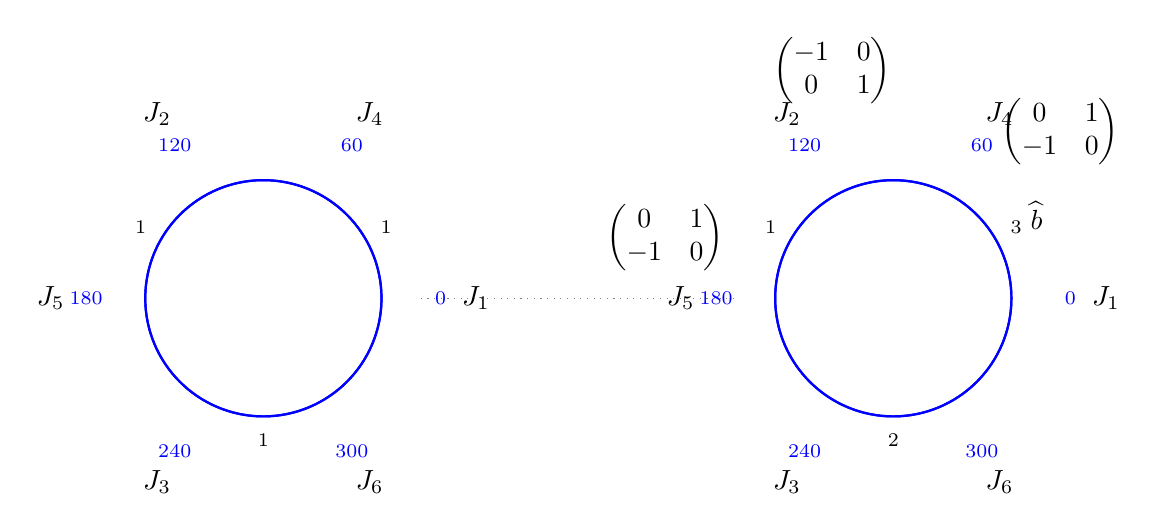
\begin{tikzpicture}
    % Left side: Before Fourier transform
    \begin{scope}[shift={(-4,0)}, scale=1.5]
        \draw[blue, thick] (0,0) circle(1);
        \foreach \i in {1,2,3} {
            \draw[blue, thick] (120*\i:1) arc[start angle=120*\i, end angle=120*\i+60, radius=1];
            \draw[blue, thick] (120*\i+60:1) arc[start angle=120*\i+60, end angle=120*\i+120, radius=1];
            \node at (120*\i+30:1.2) {\(\scriptstyle 1\)};
        }
        \foreach \i/\j in {J_1/0, J_2/120, J_3/240, J_4/60, J_5/180, J_6/300} {
            \node[blue] at (\j:1.5) {\(\scriptstyle \j\)};
            \node at (\j:1.8) {\(\i\)};
        }
    \end{scope}
    
    % Right side: After Fourier transform
    \begin{scope}[shift={(4,0)}, scale=1.5]
        \draw[blue, thick] (0,0) circle(1);
        \foreach \i in {1,2,3} {
            \draw[blue, thick] (120*\i:1) arc[start angle=120*\i, end angle=120*\i+60, radius=1];
            \draw[blue, thick] (120*\i+60:1) arc[start angle=120*\i+60, end angle=120*\i+120, radius=1];
            \node at (120*\i+30:1.2) {\(\scriptstyle \i\)};
        }
        \foreach \i/\j in {J_1/0, J_2/120, J_3/240, J_4/60, J_5/180, J_6/300} {
            \node[blue] at (\j:1.5) {\(\scriptstyle \j\)};
            \node at (\j:1.8) {\(\i\)};
        }
        \node at (30:1.4) {\(\widehat{b}\)};
        \node at (45:2) {\(\begin{pmatrix} 0 & 1 \\ -1 & 0 \end{pmatrix}\)};
        \node at (105:2) {\(\begin{pmatrix} -1 & 0 \\ 0 & 1 \end{pmatrix}\)};
        \node at (165:2) {\(\begin{pmatrix} 0 & 1 \\ -1 & 0 \end{pmatrix}\)};
    \end{scope}
    
    % Connectors
    \draw[dotted, gray] (-2,0) -- (2,0);
\end{tikzpicture}

\end{document}